\documentclass{standalone}
\usepackage{tikz}
\usetikzlibrary{patterns, positioning}


\begin{document}
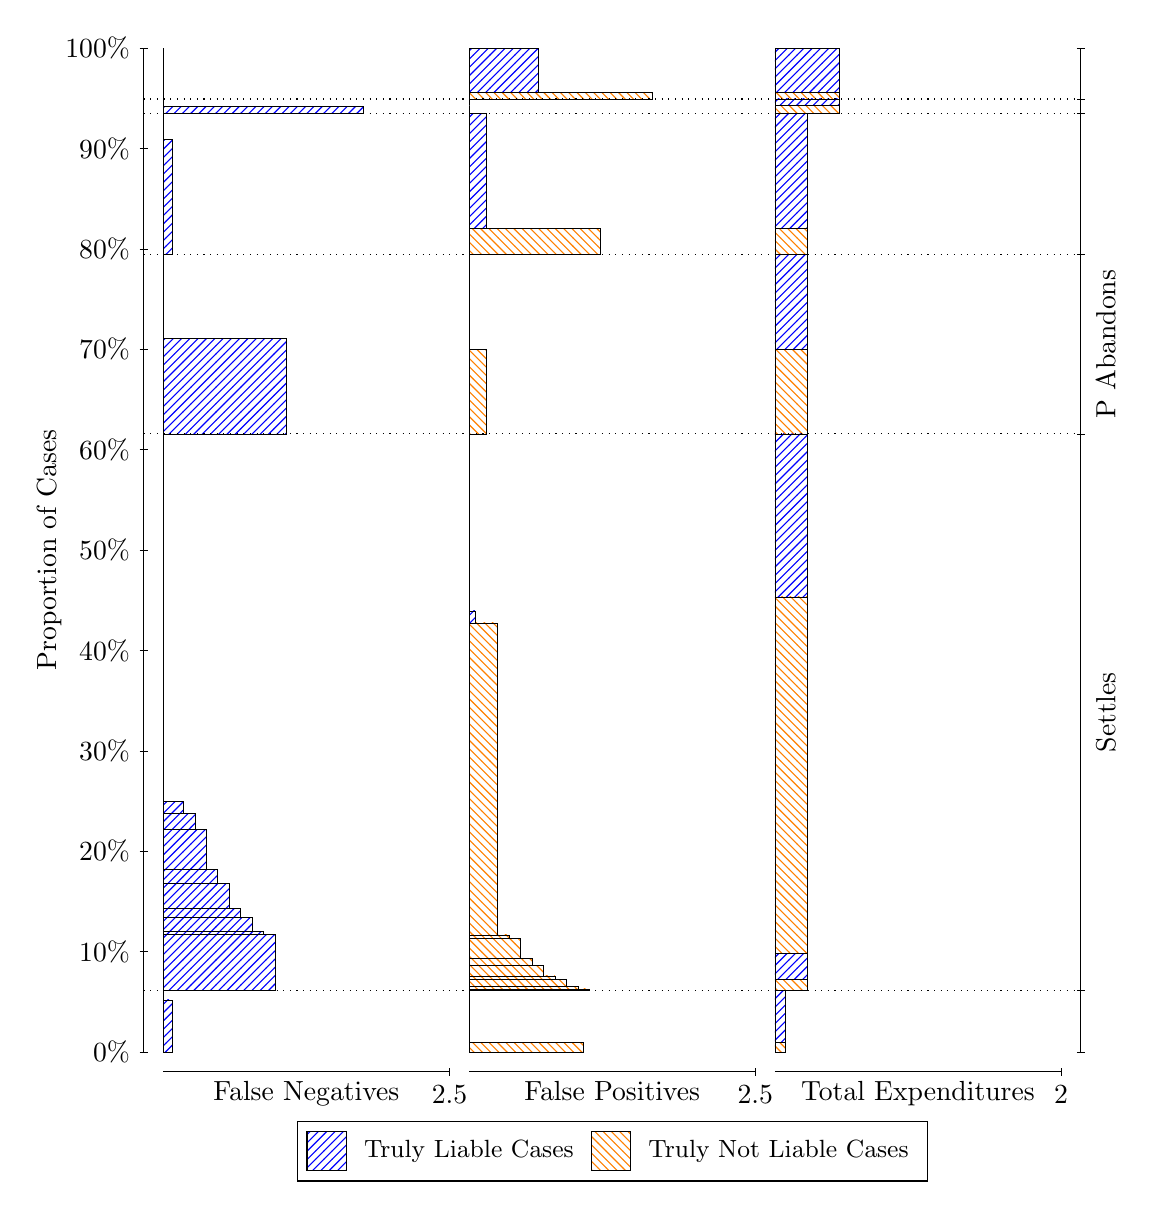
\begin{tikzpicture}
\draw[black, very thin] (1.5,1.75) -- (1.5,14.5);
\node[rotate=90, text=black, anchor=center] at (0.3, 8.125) {Proportion of Cases};
\draw[black, very thin] (1.45,1.75) -- (1.55,1.75);
\node[text=black, anchor=east] at (1.45, 1.75) {0\%};
\draw[black, very thin] (1.45,3.025) -- (1.55,3.025);
\node[text=black, anchor=east] at (1.45, 3.025) {10\%};
\draw[black, very thin] (1.45,4.3) -- (1.55,4.3);
\node[text=black, anchor=east] at (1.45, 4.3) {20\%};
\draw[black, very thin] (1.45,5.575) -- (1.55,5.575);
\node[text=black, anchor=east] at (1.45, 5.575) {30\%};
\draw[black, very thin] (1.45,6.85) -- (1.55,6.85);
\node[text=black, anchor=east] at (1.45, 6.85) {40\%};
\draw[black, very thin] (1.45,8.125) -- (1.55,8.125);
\node[text=black, anchor=east] at (1.45, 8.125) {50\%};
\draw[black, very thin] (1.45,9.4) -- (1.55,9.4);
\node[text=black, anchor=east] at (1.45, 9.4) {60\%};
\draw[black, very thin] (1.45,10.675) -- (1.55,10.675);
\node[text=black, anchor=east] at (1.45, 10.675) {70\%};
\draw[black, very thin] (1.45,11.95) -- (1.55,11.95);
\node[text=black, anchor=east] at (1.45, 11.95) {80\%};
\draw[black, very thin] (1.45,13.225) -- (1.55,13.225);
\node[text=black, anchor=east] at (1.45, 13.225) {90\%};
\draw[black, very thin] (1.45,14.5) -- (1.55,14.5);
\node[text=black, anchor=east] at (1.45, 14.5) {100\%};

\draw[black, very thin] (13.4,1.75) -- (13.4,14.5);
\draw[black, very thin] (13.35,1.75) -- (13.45,1.75);
\node[anchor=west] at (13.35, 1.75) {};
\draw[black, very thin] (13.35,2.5315) -- (13.45,2.5315);
\node[anchor=west] at (13.35, 2.5315) {};
\draw[black, very thin] (13.35,9.5989) -- (13.45,9.5989);
\node[anchor=west] at (13.35, 9.5989) {};
\draw[black, very thin] (13.35,11.879) -- (13.45,11.879);
\node[anchor=west] at (13.35, 11.879) {};
\draw[black, very thin] (13.35,13.67) -- (13.45,13.67);
\node[anchor=west] at (13.35, 13.67) {};
\draw[black, very thin] (13.35,13.853) -- (13.45,13.853);
\node[anchor=west] at (13.35, 13.853) {};
\draw[black, very thin] (13.35,14.5) -- (13.45,14.5);
\node[anchor=west] at (13.35, 14.5) {};

\draw[black, very thin, pattern color=blue, pattern=north east lines] (1.75,1.75) rectangle (1.859,2.4107);
\draw[black, very thin, pattern color=orange, pattern=north west lines] (1.75,2.4107) rectangle (1.75,2.5315);
\draw[black, very thin, pattern color=blue, pattern=north east lines] (1.75,2.5315) rectangle (3.167,3.2434);
\draw[black, very thin, pattern color=blue, pattern=north east lines] (1.75,3.2434) rectangle (3.0217,3.2836);
\draw[black, very thin, pattern color=blue, pattern=north east lines] (1.75,3.2836) rectangle (2.8763,3.4636);
\draw[black, very thin, pattern color=blue, pattern=north east lines] (1.75,3.4636) rectangle (2.731,3.5752);
\draw[black, very thin, pattern color=blue, pattern=north east lines] (1.75,3.5752) rectangle (2.5857,3.8889);
\draw[black, very thin, pattern color=blue, pattern=north east lines] (1.75,3.8889) rectangle (2.4403,4.0734);
\draw[black, very thin, pattern color=blue, pattern=north east lines] (1.75,4.0734) rectangle (2.295,4.5766);
\draw[black, very thin, pattern color=blue, pattern=north east lines] (1.75,4.5766) rectangle (2.1497,4.7774);
\draw[black, very thin, pattern color=blue, pattern=north east lines] (1.75,4.7774) rectangle (2.0043,4.9299);
\draw[black, very thin, pattern color=orange, pattern=north west lines] (1.75,4.9299) rectangle (1.75,9.5989);
\draw[black, very thin, pattern color=blue, pattern=north east lines] (1.75,9.5989) rectangle (3.3123,10.808);
\draw[black, very thin, pattern color=orange, pattern=north west lines] (1.75,10.808) rectangle (1.75,11.879);
\draw[black, very thin, pattern color=blue, pattern=north east lines] (1.75,11.879) rectangle (1.859,13.341);
\draw[black, very thin, pattern color=orange, pattern=north west lines] (1.75,13.341) rectangle (1.75,13.67);
\draw[black, very thin, pattern color=blue, pattern=north east lines] (1.75,13.67) rectangle (4.2933,13.755);
\draw[black, very thin, pattern color=orange, pattern=north west lines] (1.75,13.755) rectangle (1.75,13.853);
\draw[black, very thin, pattern color=orange, pattern=north west lines] (1.75,13.853) rectangle (1.75,13.941);
\draw[black, very thin, pattern color=blue, pattern=north east lines] (1.75,13.941) rectangle (1.75,14.5);
\draw[black, very thin, pattern color=orange, pattern=north west lines] (5.6333,1.75) rectangle (7.0867,1.8708);
\draw[black, very thin, pattern color=blue, pattern=north east lines] (5.6333,1.8708) rectangle (5.6333,2.5315);
\draw[black, very thin, pattern color=orange, pattern=north west lines] (5.6333,2.5315) rectangle (7.1593,2.5506);
\draw[black, very thin, pattern color=orange, pattern=north west lines] (5.6333,2.5506) rectangle (7.014,2.5848);
\draw[black, very thin, pattern color=orange, pattern=north west lines] (5.6333,2.5848) rectangle (6.8687,2.6737);
\draw[black, very thin, pattern color=orange, pattern=north west lines] (5.6333,2.6737) rectangle (6.7233,2.7159);
\draw[black, very thin, pattern color=orange, pattern=north west lines] (5.6333,2.7159) rectangle (6.578,2.8496);
\draw[black, very thin, pattern color=orange, pattern=north west lines] (5.6333,2.8496) rectangle (6.4327,2.8541);
\draw[black, very thin, pattern color=orange, pattern=north west lines] (5.6333,2.8541) rectangle (6.4327,2.9386);
\draw[black, very thin, pattern color=orange, pattern=north west lines] (5.6333,2.9386) rectangle (6.2873,3.1936);
\draw[black, very thin, pattern color=orange, pattern=north west lines] (5.6333,3.1936) rectangle (6.142,3.2361);
\draw[black, very thin, pattern color=orange, pattern=north west lines] (5.6333,3.2361) rectangle (5.9967,7.2006);
\draw[black, very thin, pattern color=blue, pattern=north east lines] (5.6333,7.2006) rectangle (5.706,7.3531);
\draw[black, very thin, pattern color=blue, pattern=north east lines] (5.6333,7.3531) rectangle (5.6333,9.5989);
\draw[black, very thin, pattern color=orange, pattern=north west lines] (5.6333,9.5989) rectangle (5.8513,10.67);
\draw[black, very thin, pattern color=blue, pattern=north east lines] (5.6333,10.67) rectangle (5.6333,11.879);
\draw[black, very thin, pattern color=orange, pattern=north west lines] (5.6333,11.879) rectangle (7.3047,12.207);
\draw[black, very thin, pattern color=blue, pattern=north east lines] (5.6333,12.207) rectangle (5.8513,13.67);
\draw[black, very thin, pattern color=orange, pattern=north west lines] (5.6333,13.67) rectangle (5.6333,13.768);
\draw[black, very thin, pattern color=blue, pattern=north east lines] (5.6333,13.768) rectangle (5.6333,13.853);
\draw[black, very thin, pattern color=orange, pattern=north west lines] (5.6333,13.853) rectangle (7.9587,13.941);
\draw[black, very thin, pattern color=blue, pattern=north east lines] (5.6333,13.941) rectangle (6.5053,14.5);
\draw[black, very thin, pattern color=orange, pattern=north west lines] (9.5167,1.75) rectangle (9.6529,1.8708);
\draw[black, very thin, pattern color=blue, pattern=north east lines] (9.5167,1.8708) rectangle (9.6529,2.5315);
\draw[black, very thin, pattern color=orange, pattern=north west lines] (9.5167,2.5315) rectangle (9.9254,2.6698);
\draw[black, very thin, pattern color=blue, pattern=north east lines] (9.5167,2.6698) rectangle (9.9254,2.9979);
\draw[black, very thin, pattern color=orange, pattern=north west lines] (9.5167,2.9979) rectangle (9.9254,7.5288);
\draw[black, very thin, pattern color=blue, pattern=north east lines] (9.5167,7.5288) rectangle (9.9254,9.5989);
\draw[black, very thin, pattern color=orange, pattern=north west lines] (9.5167,9.5989) rectangle (9.9254,10.67);
\draw[black, very thin, pattern color=blue, pattern=north east lines] (9.5167,10.67) rectangle (9.9254,11.879);
\draw[black, very thin, pattern color=orange, pattern=north west lines] (9.5167,11.879) rectangle (9.9254,12.207);
\draw[black, very thin, pattern color=blue, pattern=north east lines] (9.5167,12.207) rectangle (9.9254,13.67);
\draw[black, very thin, pattern color=orange, pattern=north west lines] (9.5167,13.67) rectangle (10.334,13.768);
\draw[black, very thin, pattern color=blue, pattern=north east lines] (9.5167,13.768) rectangle (10.334,13.853);
\draw[black, very thin, pattern color=orange, pattern=north west lines] (9.5167,13.853) rectangle (10.334,13.941);
\draw[black, very thin, pattern color=blue, pattern=north east lines] (9.5167,13.941) rectangle (10.334,14.5);
\draw[black, dotted] (1.5,2.5315) -- (13.4,2.5315);
\draw[black, dotted] (1.5,9.5989) -- (13.4,9.5989);
\draw[black, dotted] (1.5,11.879) -- (13.4,11.879);
\draw[black, dotted] (1.5,13.67) -- (13.4,13.67);
\draw[black, dotted] (1.5,13.853) -- (13.4,13.853);
\draw[black, very thin] (1.75,1.5) -- (5.3833,1.5);
\node[text=black, anchor=north] at (3.5667, 1.5) {False Negatives};
\draw[black, very thin] (5.3833,1.45) -- (5.3833,1.55);
\node[text=black, anchor=north] at (5.3833, 1.45) {2.5};

\draw[black, very thin] (5.6333,1.5) -- (9.2667,1.5);
\node[text=black, anchor=north] at (7.45, 1.5) {False Positives};
\draw[black, very thin] (9.2667,1.45) -- (9.2667,1.55);
\node[text=black, anchor=north] at (9.2667, 1.45) {2.5};

\draw[black, very thin] (9.5167,1.5) -- (13.15,1.5);
\node[text=black, anchor=north] at (11.333, 1.5) {Total Expenditures};
\draw[black, very thin] (13.15,1.45) -- (13.15,1.55);
\node[text=black, anchor=north] at (13.15, 1.45) {2};


\node[text=black, centered, rotate=90] at (13.72, 6.0652) {Settles};
\node[text=black, centered, rotate=90] at (13.72, 10.739) {P Abandons};




\draw (7.449999999999999,1.5) node[draw=none] (baseCoordinate) {};
\begin{scope}[align=center]
        \matrix[scale=0.5, draw=black, below=0.5cm of baseCoordinate, nodes={draw}, column sep=0.1cm]{
            \node[rectangle, draw, minimum width=0.5cm, minimum height=0.5cm, pattern color=blue, pattern=north east lines] {}; &
            \node[draw=none, font=\small, text=black] (B) {Truly Liable Cases}; &
            \node[rectangle, draw, minimum width=0.5cm, minimum height=0.5cm, pattern color=orange, pattern=north west lines] {}; &
            \node[draw=none, font=\small, text=black] (B) {Truly Not Liable Cases}; \\
            };
\end{scope}

\end{tikzpicture}
\end{document}